% Made up for the tikra benchmark.
\usetikzlibrary{circuits.ee.IEC}
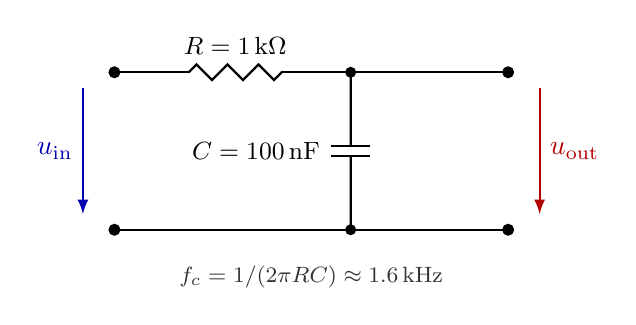
\begin{tikzpicture}[circuit ee IEC, thick, every info/.style={font=\small},
    set resistor graphic=var resistor IEC graphic]
  \node[contact] (in1) at (0,2) {};
  \node[contact] (in2) at (0,0) {};
  \node[contact] (out1) at (5,2) {};
  \node[contact] (out2) at (5,0) {};
  \draw (in1) to [resistor={info={$R=1\,\mathrm{k\Omega}$}}] (3,2) -- (out1);
  \draw (3,2) to [capacitor={info'={$C=100\,\mathrm{nF}$}}] (3,0);
  \draw (in2) -- (out2);
  \fill (3,2) circle (2pt) (3,0) circle (2pt);
  \draw[-latex, blue!70!black] (-0.4,1.8) -- node[left] {$u_\mathrm{in}$} (-0.4,0.2);
  \draw[-latex, red!70!black] (5.4,1.8) -- node[right] {$u_\mathrm{out}$} (5.4,0.2);
  \node[font=\footnotesize, gray!40!black] at (2.5,-0.6) {$f_c = 1/(2\pi RC) \approx 1.6\,\mathrm{kHz}$};
\end{tikzpicture}
